%\RequirePackage{atbegshi}
\documentclass[french]{beamer}
\usepackage{etex}

\usepackage[beamer,euler, utf8x]{preambuleTrm}



\usepackage{iwona}


\mode<presentation>
{
  %\usetheme{Bergen}%Montpellier,Madrid}
  % or ...Frankfurt, 
  \usetheme{Montpellier}

  %\setbeamercovered{highly dynamic}
  % or whatever (possibly just delete it)
  \usefonttheme{progressbar}
%  \useoutertheme{progressbar}
  %\useinnertheme{progressbar}
 % \progressbaroptions{% titlepage=normal,
  %  imagename=/home/moi/Photos/Maths/prisoner
%}
}

%\usepackage{elephantbird}
\newcommand\MyBox[2][XXX]{%
  \fbox{\tabular[b]{C{#1}} #2 \endtabular}}

\setbeamertemplate{footline}[frame number]
\beamertemplatenavigationsymbolsempty

%\usepackage[french,vlined,boxed]{algorithm2e}
\usepackage{bookmark,multido}
%\usepackage{xlop}

\ifpdf \DeclareGraphicsRule{*}{mps}{*}{} \fi



% \usepackage{tikz, pgfkeys, pgfopts, xstring}
% \usetikzlibrary{automata,fit,trees,matrix,arrows,decorations.markings,shapes,arrows,chains,positioning,intersections,backgrounds,calc,through,mindmap,shadows,patterns, decorations.pathmorphing}

% \usepackage{tkz-linknodes}

% \usepackage{tkz-graph,tikz-uml, tkz-berge}
% \input{patch-tkz-graph}
% \usepackage{tikz-qtree}



\usepackage{tikz}
\usetikzlibrary{automata,fit,trees,shapes.arrows,chains,positioning,intersections,backgrounds,calc,matrix,arrows,decorations.pathmorphing}
\newcommand{\myunit}{1.1cm}
\usepackage{tkz-graph, tkz-berge}
\input{patch-tkz-graph}
\usepackage{tikz-qtree}
%\usepackage{circuitikz}
%\usepackage{Karnaugh}
%\usepackage[autolanguage]{numprint}

\usepackage{tkz-linknodes}



\usepackage[underline=true,rounded corners=false]{pgf-umlsd}

\hypersetup{pdfpagemode=FullScreen}

\usepackage[detect-all]{siunitx}

\usepackage{caption}
\captionsetup{labelformat=empty,font=footnotesize}

\usepackage[square]{daedale}
\bibliographystyle{cyclope}


\usepackage{algo}

\renewcommand{\algocommentfont}{\tiny\ttfamily\itshape}
\renewcommand{\algokeywordfont}{\small\ttfamily}
\renewcommand{\algotextfont}{\footnotesize\ttfamily}
\newtheorem{exercice}{Exercice}


\setlength{\columnseprule}{0pt}

%\setlength{\parskip}{0pt}


\graphicspath{{/home/moi/Photos/Maths/small/}{/home/moi/IUT/Figures/}{/home/moi/VISA_III/figures_visa/}{/home/moi/Lycee/TDmaple/2006_7/}{/home/moi/Figures/Arbres_Graphes/}{/home/moi/Figures/FigSTI/}{/home/moi/Figures/FigMaple/}{/home/moi/Photos/Maths/}{/home/moi/Photos/Tehessin/}{/home/moi/Figures/FigSTI/}{/home/moi/Figures/FigSeconde/}{/home/moi/Lycee/Informatique/XCAS/2008_9/}{/home/moi/Lycee/TDmaple/2008_9/}{/home/moi/IUT/Thierry/Conversions/}{/home/moi/Photos/informathix/}{/home/moi/Lycee/Informatique/PafAlgo/}{/home/moi/Figures/figuresAlice/}{/home/moi/Figures/FigSeconde/}{/home/moi/Biocam/robot/}{/home/moi/Biocam/CoursIni3d/}{/home/moi/Biocam/central/figures/}{/home/moi/Biocam/central/}{/home/moi/IUT/INFO2/Images/}{/home/moi/IUT/INFO2/2011_12/graphes/}{/home/moi/IUT/INFO1/CM1/}{/home/moi/Figures/figuresTS/}{/home/moi/Photos/Tehessin/}{/home/moi/Figures/FigSTI/}{/home/moi/Alice/figures3/}{/home/moi/Alice/figures3/newcourbes/}{/home/moi/Alice/figures/}{/home/moi/Figures/figuresAlice/}{/home/moi/Photos/Maths/}{/home/moi/Lycee/TS/}{/home/moi/Lycee/TS/2009_10/}{/home/moi/Figures/FigMaple/}{/home/moi/Figures/figuresTS/newcourbes/}{/home/moi/Figures/FigEspace/}{/home/moi/PROG/HASKELL/FLOAT/}{/home/moi/LYCEE/LIL/4e/2016_17/Images/}{/home/moi/LYCEE/LIL/2nde/2016_17/Images/}{/home/moi/LYCEE/LIL/2nde/2016_17/fonctions/}{/home/moi/LYCEE/LIL/1S/2016_17/Images/}{/home/moi/LYCEE/LIL/1S/2016_17/Images/}{/home/moi/LYCEE/LIL/1S/2016_17/suites/suites1es/}{/home/moi/LYCEE/LIL/1S/2016_17/trigo/}{/home/moi/Photos/Maths/CAPTURES_TI/Suites/}{/home/moi/LYCEE/FIGURES/}{/home/moi/UCO/L1/ANGERS2018/Images/}}



\setcounter{tocdepth}{2} %\setcounter{page}{0}




\usepackage{fdsymbol}





\setbeamercolor{block title}{use=structure,fg=black,bg=blue!55!white}
\setbeamercolor{block body}{use=structure,fg=black,bg=blue!10!white}


\setbeamercolor{block title example}{use=structure,fg=black,bg=green!55!white}
\setbeamercolor{block body example}{use=structure,fg=black,bg=green!10!white}

\setbeamercolor{block title alerted}{use=structure,fg=black,bg=red!55!white}
\setbeamercolor{block body alerted}{use=structure,fg=black,bg=red!10!white}



\setbeamerfont{block body}{size*={10}{12}}
\setbeamerfont{block body alerted}{size*={10}{12}}
\setbeamerfont{block body example}{size*={10}{12}}


%\renewenvironment{exercise}{\begin{exampleblock}{Recherche}}{\end{exampleblock}}

\usepackage{scalefnt}
\setbeamertemplate{theorems}[normal size]


\begin{document}


\title[]% (optional, use only with long paper titles)
{INFORMATIQUE}

\subtitle{Introduction}

\author[] % (optional, use only with lots of authors)
{Guillaume CONNAN }
% - Give the names in the same order as the appear in the paper.
% - Use the inst{?} command only if the authors have different
%   affiliation.


\institute{Lycée Notre-Dame - 2$^{nde}$}% (optional, but mostly needed)

\logo{\includegraphics[width=0.1\textwidth]{logondr}}

%\logo{\includegraphics[scale=0.15]{big_connan}}

\date[] % (optional, should be abbreviation of conference name)
{\today{}}
% - Either use conference name or its abbreviation.
% - Not really informative to the audience, more for people (including
%   yourself) who are reading the slides online

\subject{ }



\beamerdefaultoverlayspecification{<+->}


\AtBeginSubsection[]
{\scriptsize
  \begin{frame}<beamer>
    \frametitle{Sommaire}
 {\tiny
\begin{multicols}{2}
    \tableofcontents[currentsection,currentsubsection]
       \end{multicols}
}

  \end{frame}
}





\AtBeginSection[]
{
  \begin{frame}<beamer>
    \frametitle{Sommaire}
 {\scriptsize
\begin{multicols}{2}
    \tableofcontents[currentsection]
       \end{multicols}
}

  \end{frame}
}


% If you wish to uncover everything in a step-wise fashion, uncomment
% the following command: 

\beamerdefaultoverlayspecification{<+->}




\newcommand{\TR}{\mathcal{T}}


\begin{frame}
%\ThisCenterWallPaper{1}{logoiremBigInv}
 \Large \titlepage 
\end{frame}

\begin{frame}
 \frametitle{Sommaire}
{\scriptsize
\begin{multicols}{2} 
 \tableofcontents
\end{multicols}
}

 
 \end{frame}

\normalsize


























% début



\section{SNT???}

\begin{frame}[fragile]{Informatique}
\protect\hypertarget{informatique}{}


Première chose à faire : oublier cette appellation idiote\ldots{}
\pause ScienceS ? \pause Numériques ? \pause et technologie ????
\pause
Non !! Vous avez des cours d'histoire, d'anglais, de maths. Aujourd'hui
nous commençons un nouveau cours d'\textbf{INFORMATIQUE}.
\pause
Peu de gens sont au courant mais il y a en effet un nouveau truc qui
vient de sortir et qui s'appelle \pause \emph{in-for-ma-tique}.


\end{frame}

\begin{frame}
   La France vient
de le découvrir et l'introduit à l'école:\pause
\begin{figure}
\centering
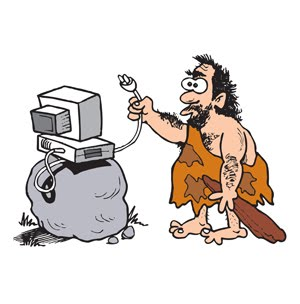
\includegraphics{./caveman.jpg}
\caption{La France et l'enseignement de l'informatique}
\end{figure}
\end{frame}



\begin{frame}
Pendant ce temps, ailleurs dans le monde\ldots{}
\pause
\begin{figure}
\centering
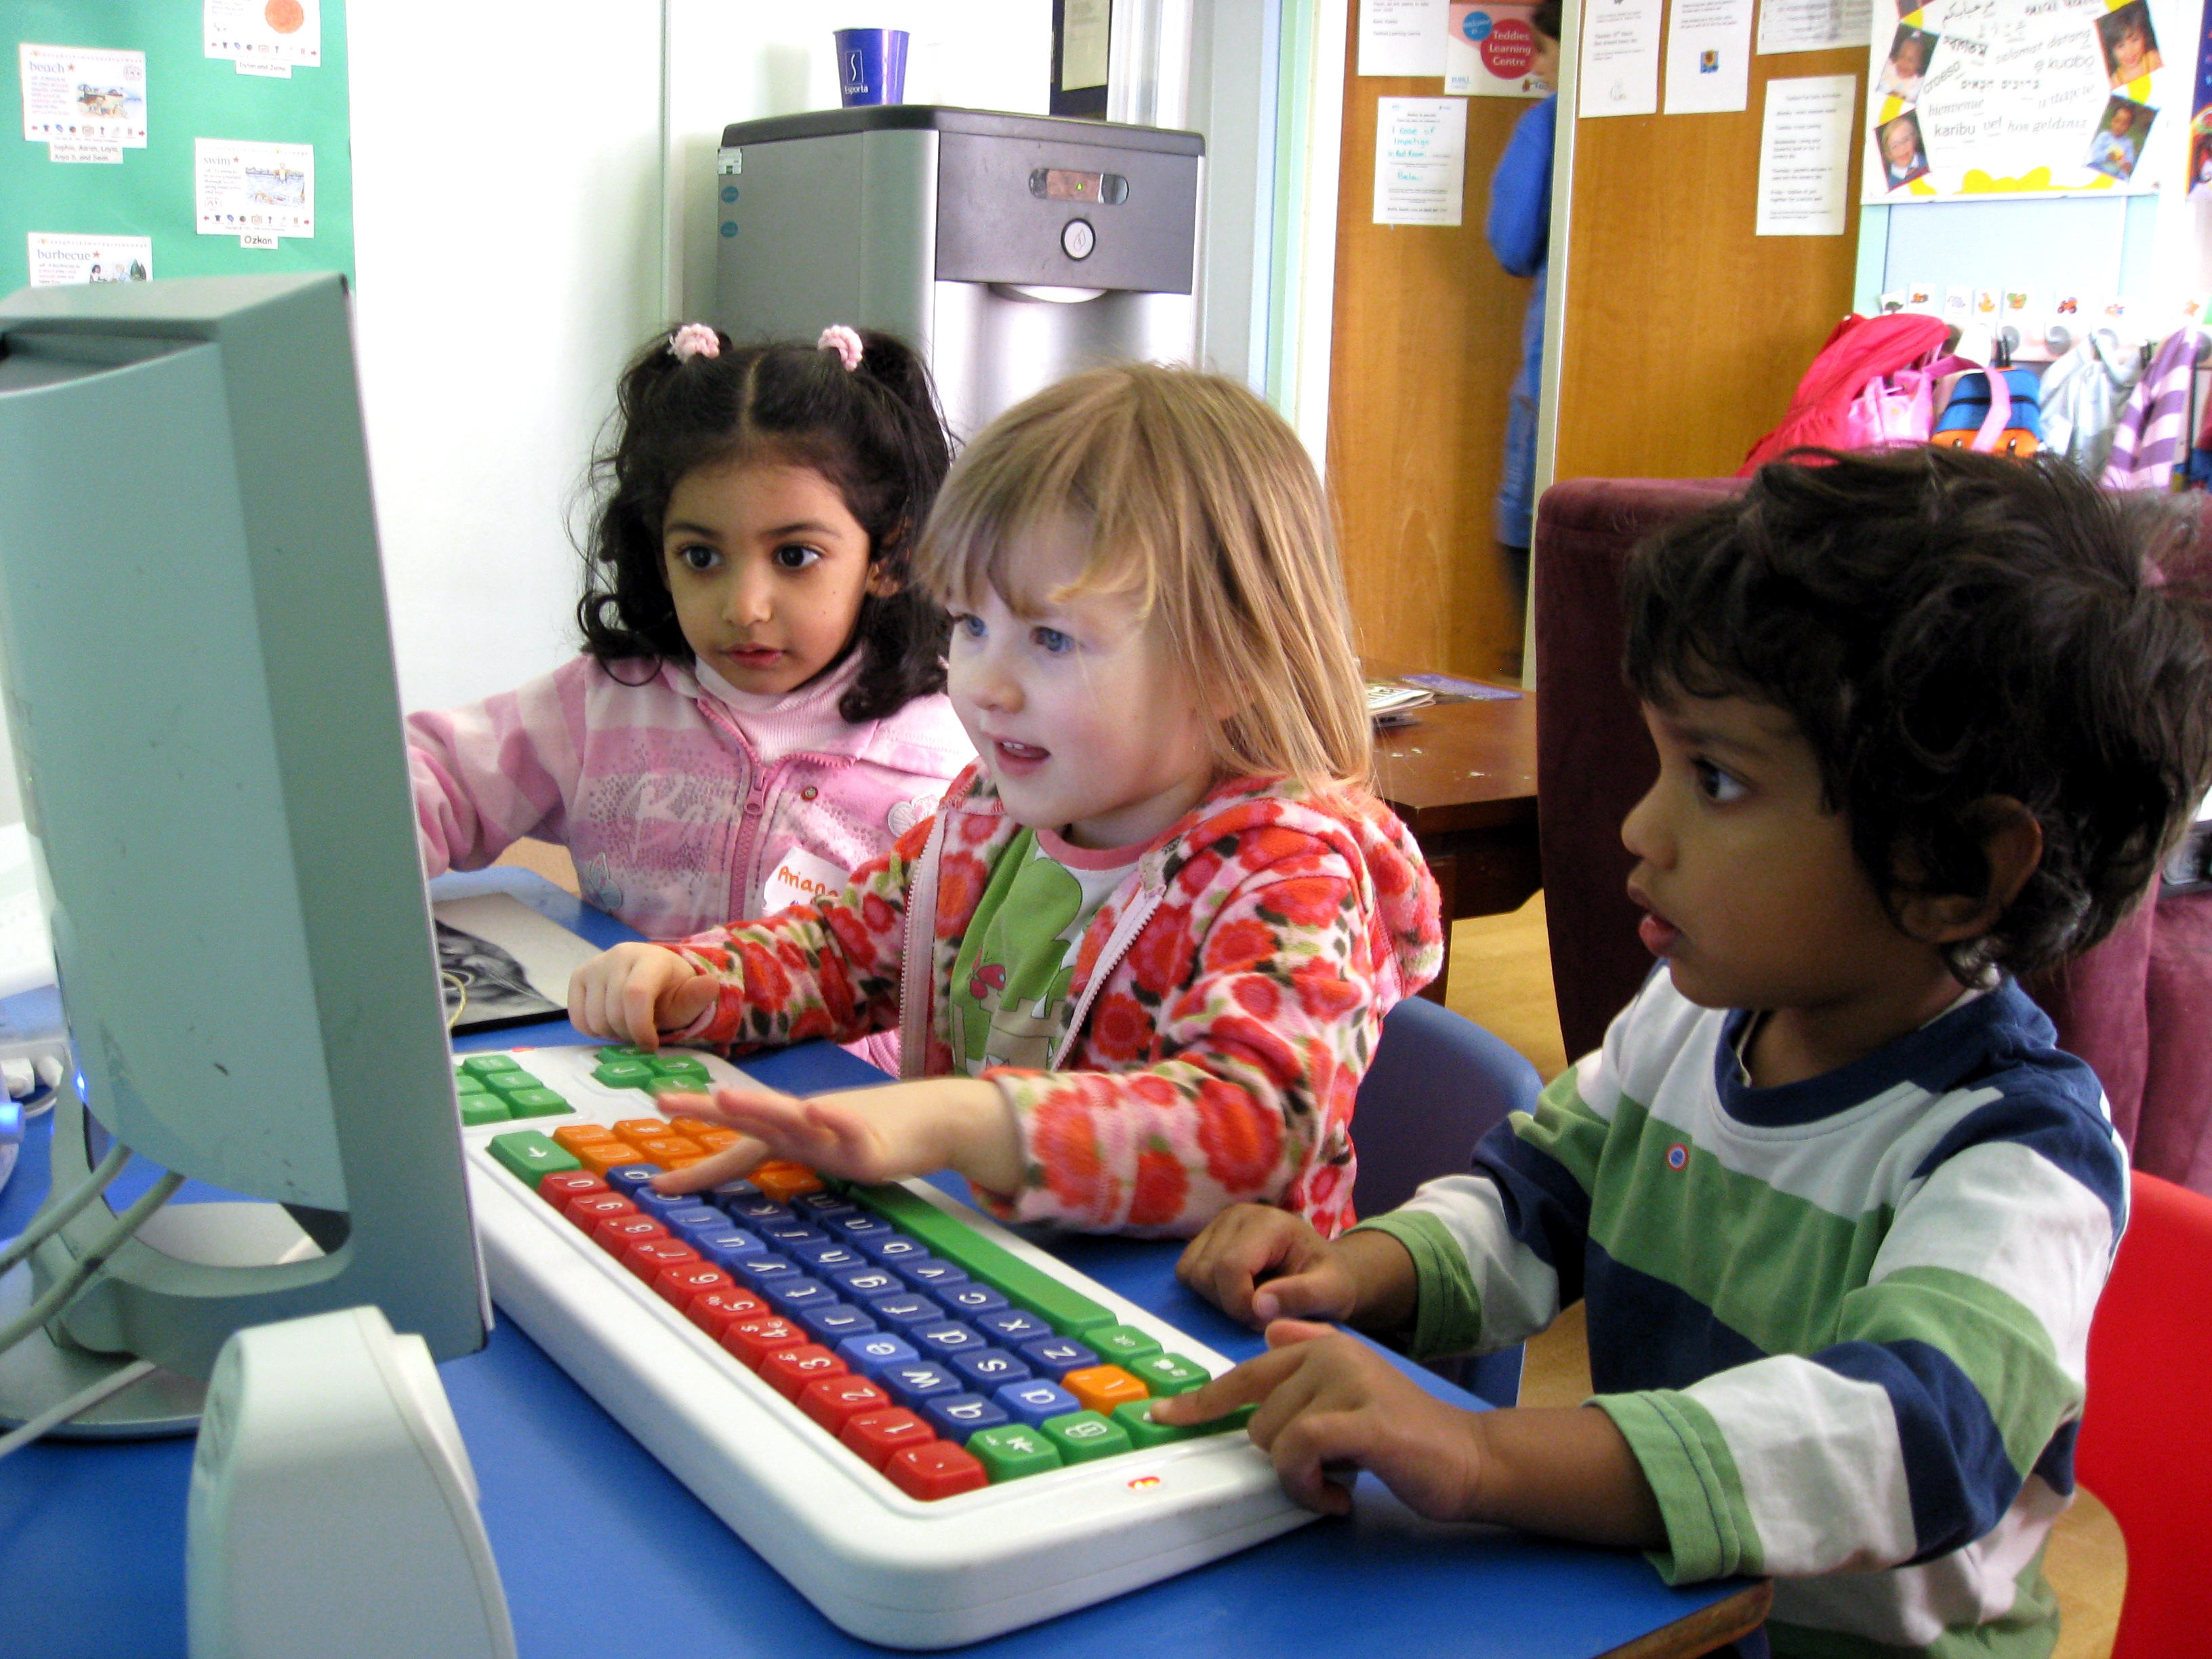
\includegraphics[height=0.7\textheight]{./kids.JPG}
\end{figure}

\end{frame}




\section{Informatique ???}

\begin{frame}
Au fait, l'informatique c'est quoi ?

C'est par exemple ça:
 \begin{center}
\href{https://www.youtube.com/embed/jpfHxfF-Kno}{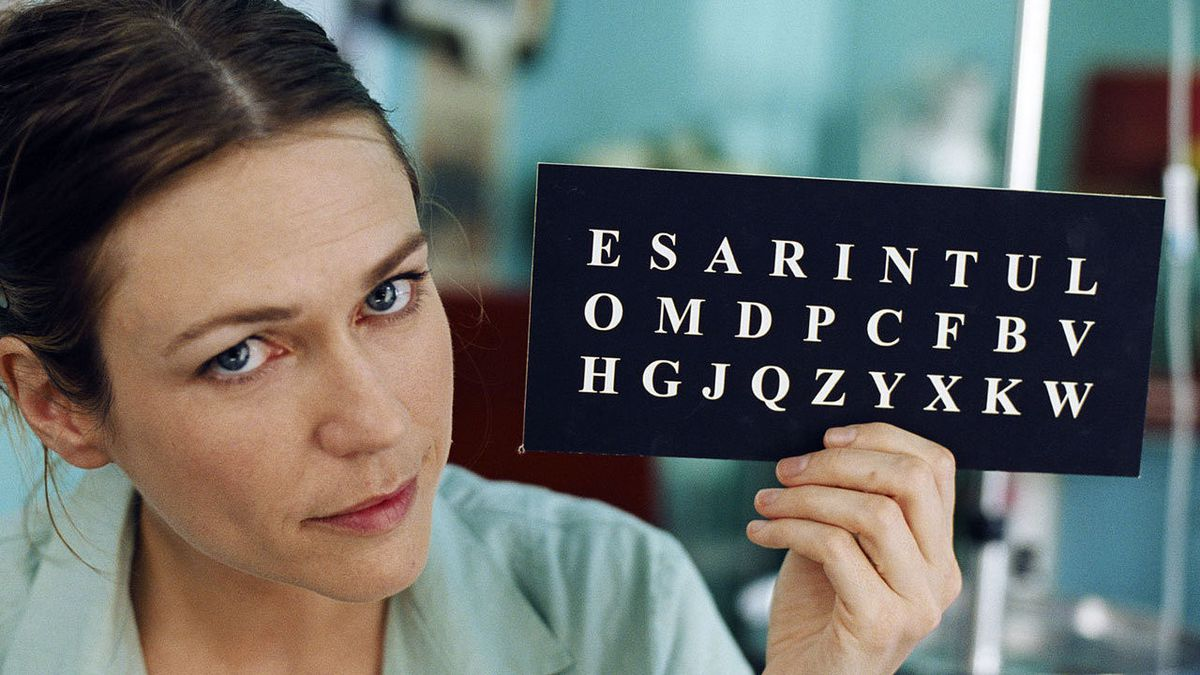
\includegraphics[height=0.7\textheight]{./papillon.jpg}}
\end{center}
\end{frame}

\begin{frame}
ou en version plus blockbuster:
 \begin{center}
\href{https://www.youtube.com/embed/ffB0Je-xjKg}{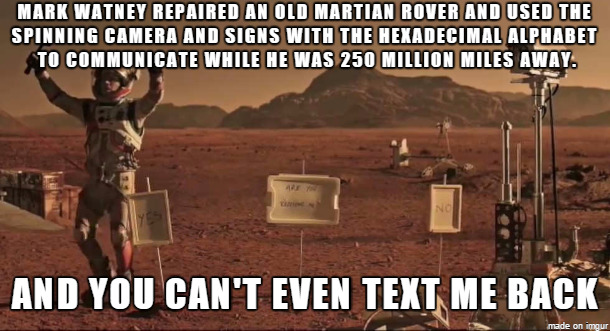
\includegraphics[height=0.7\textheight]{./martian.jpg}}
\end{center}
\end{frame}

\begin{frame}
L'\textbf{informati}que c'est LΑ \emph{SCIENCΕ} DΕ
L'\textbf{INFORMATI}ON
\end{frame}

\begin{frame}
Les physicien(ne)s traitent d'énergie, d'ondes, de matières:

\begin{itemize}
\item 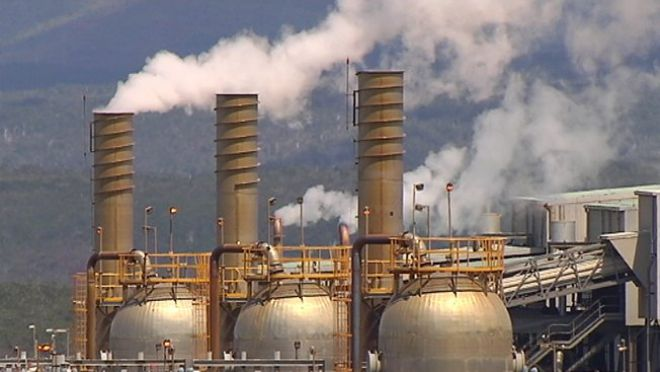
\includegraphics[height=0.4\textheight]{./usine.jpg}

\item 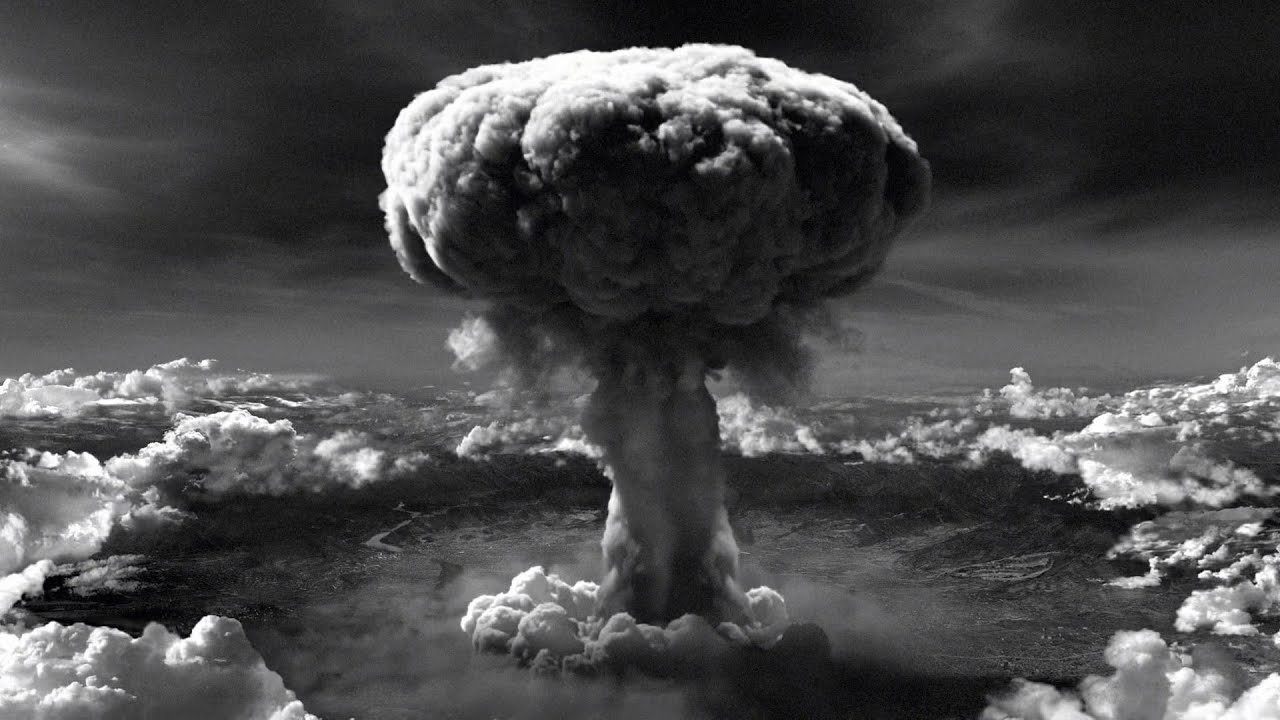
\includegraphics[height=0.4\textheight]{./hiroshima.jpg}
\end{itemize}



Les informaticien(ne)s traitent d'information.

\end{frame}

\section{Pause : information ?}


\begin{frame}
  \begin{exercice}
    \begin{itemize}
    \item Choisissez un nombre entre 0 et 127.

\item Je peux poser autant de questions que je veux mais vous ne pouvez
répondre que par oui ou non (et ne pas mentir\ldots{})

\item Combien de questions dois-je poser au maximum pour deviner le nombre ?

\item Je pourrais commencer par ``Est-ce 0 ? Est-ce 1 ? Est-ce 2 ?''\ldots{}
\item Y a-t-il plus efficace?
\end{itemize}
\end{exercice}
\end{frame}

\section{Computer science ?}

\begin{frame}

Edsger Dijkstra (Prix Turing 1972) :

\begin{quote}
``\emph{I don't need to waste my time with a computer just because I am
a computer scientist}''
\end{quote}

\end{frame}

\begin{frame}

Michael R. Fellows :

\begin{quote}
``\emph{Computer science is no more about computers than astronomy is
about telescopes, biology is about microscopes or chemistry is about
beakers and test tubes. Science is not about tools, it is about how we
use them and what we find out when we do.}''
\end{quote}
\end{frame}

\begin{frame}

Jean-Claude Simon :

\begin{quote}
``\emph{Négligeant ou ignorant les aspects intellectuels de
l'informatique, certains sont sincèrement convaincus que l'informatique
n'est pas une nouvelle discipline, mais seulement une nouvelle
technique.}''
\end{quote}

\end{frame}


\begin{frame}
Daniel Garric :

\begin{quote}
``\emph{Pour tout ce qui est caractérisé par l'informatique ou qui
caractérise l'informatique, l'ordinateur n'est pas toujours nécessaire.
Mais l'esprit informatique l'est, la décomposition de chaque problème
général en sous problèmes et leur réorganisation dynamique, les uns en
fonction des autres}''
\end{quote}

\end{frame}




\section{Numérique ? Digital ?}


\begin{frame}
    Du numérique digital:
  \begin{center}
    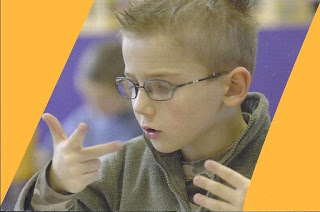
\includegraphics[height=.7\textheight]{./doigts.jpg}
  \end{center}
\end{frame}



\begin{frame}
L'atome de l'informatique est la \textbf{LOGIQUE}, pas les nombres.
Toute l'informatique se construit à partir de portes logiques,
conceptuellement comme en pratique:
\end{frame}

\begin{frame}

   \begin{center}
     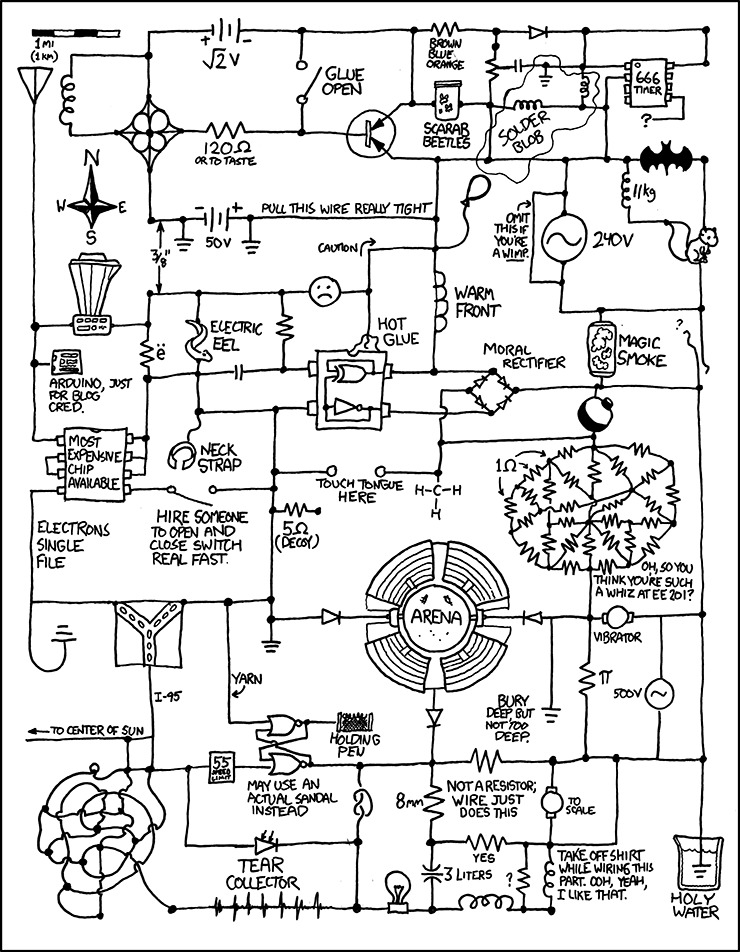
\includegraphics[height=0.9\textheight]{./circuit.jpg}
   \end{center}
 \end{frame}


\section{Beauté}

\begin{frame}
  
\begin{quote}
  {\tiny
    If you can keep your head when all about you

Are losing theirs and blaming it on you,

If you can trust yourself when all men doubt you,

But make allowance for their doubting too;

If you can wait and not be tired by waiting,

Or being lied about, don't deal in lies,

Or being hated, don't give way to hating,

And yet don't look too good, nor talk too wise:

If you can dream---and not make dreams your master;

If you can think---and not make thoughts your aim;

If you can meet with Triumph and Disaster

And treat those two impostors just the same;

If you can bear to hear the truth you've spoken

Twisted by knaves to make a trap for fools,

Or watch the things you gave your life to, broken,

And stoop and build 'em up with worn-out tools:

If you can make one heap of all your winnings

And risk it on one turn of pitch-and-toss,

And lose, and start again at your beginnings

And never breathe a word about your loss;

If you can force your heart and nerve and sinew

To serve your turn long after they are gone,

And so hold on when there is nothing in you

Except the Will which says to them: `Hold on!'

If you can talk with crowds and keep your virtue,

Or walk with Kings---nor lose the common touch,

If neither foes nor loving friends can hurt you,

If all men count with you, but none too much;

If you can fill the unforgiving minute

With sixty seconds' worth of distance run,

Yours is the Earth and everything that's in it,
And,which is more,you'll be a Man, my son!


}
\end{quote}

Rudyard Kipling

\end{frame}

\begin{frame}

\begin{quote}
Le papillon bat des ailes

Comme s'il désespérait

De ce monde.
\end{quote}

Kobayashi Issa

\end{frame}


\begin{frame}[fragile]

  \begin{pythoncode}
if x == 1:
   print(x)
else if x == 2 :
   print(x)
else if x == 3 :
   print(x)
else if x == 4 :
   print(x)
else if x == 5 :
   print(x)
else if x == 6 :
   print(x)
else if x == 7 :
   print(x)
else if x == 8 :
   print(x)
else if x == 9 :
   print(x)
else if x == 10 :
   print(x)
else:
   print(x)
\end{pythoncode}




Euuhhhh\ldots{}.

\end{frame}

\begin{frame}[fragile]

  \begin{pythoncode}
print(x)
\end{pythoncode}




Plus simple\ldots{}

Soyez DRY : \emph{Do not Repeat Yourself}

Le copier-coller : le mal incarné !

\end{frame}






\section{L'informatique a une histoire}


\begin{frame}
  \begin{center}
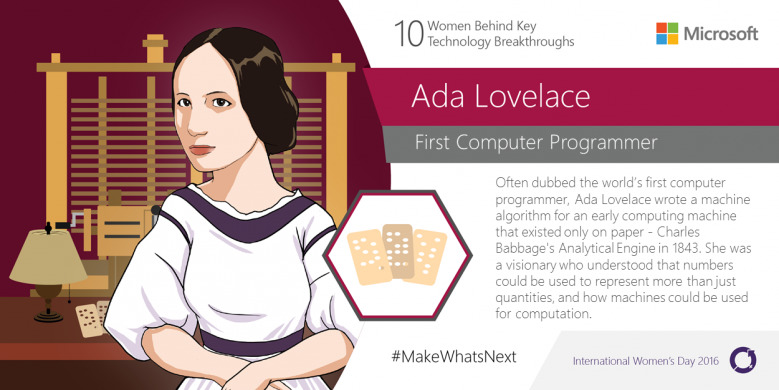
\includegraphics[height=.7\textheight]{./ada.jpg}
    
  \end{center}


\end{frame}



\section{IPad\ldots{}}

\begin{frame}
L'IPad est à l'informatique ce que ce piano est à la musique\ldots{}
 \begin{center}
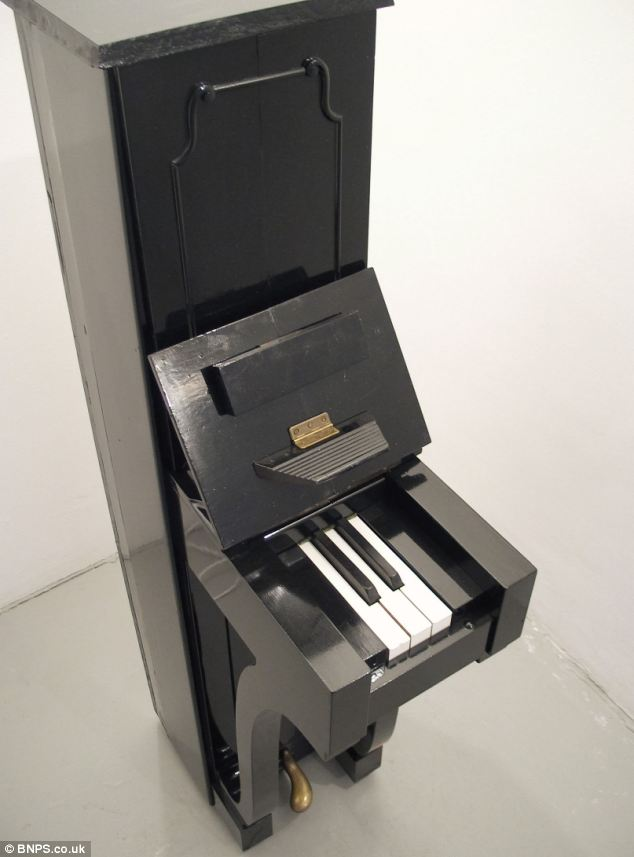
\includegraphics[height=.8\textheight]{./IpadPiano2touches.jpg}
\end{center}
\end{frame}





\section{L'informatique dans la société}

\begin{frame}
   \begin{center}
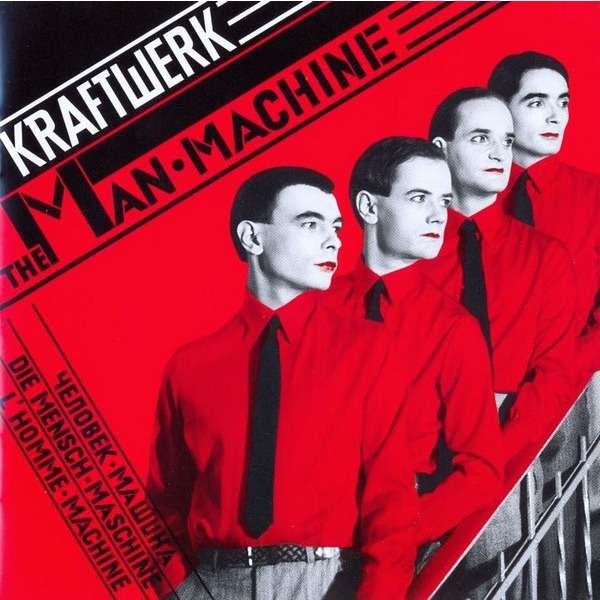
\includegraphics[height=.8\textheight]{./manmachine.jpeg}
\end{center}
\end{frame}




\section{Internet des objets}


\begin{frame}
   \begin{center}
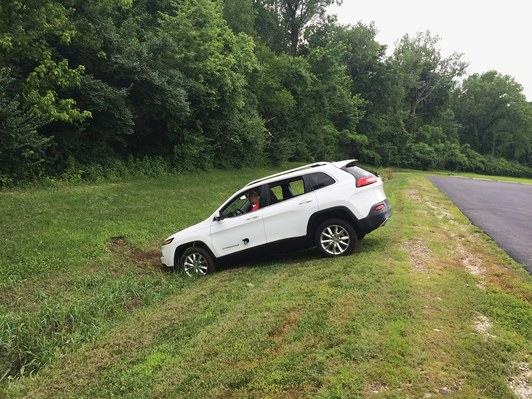
\includegraphics[height=.8\textheight]{jeep.jpg}
\end{center}
\end{frame}



\begin{frame}
   \begin{center}
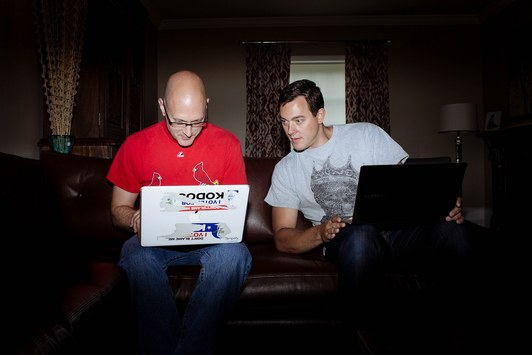
\includegraphics[height=.8\textheight]{millerval.jpg}
\end{center}
\end{frame}



\section{Des blagues}




\begin{frame}
   \begin{center}
     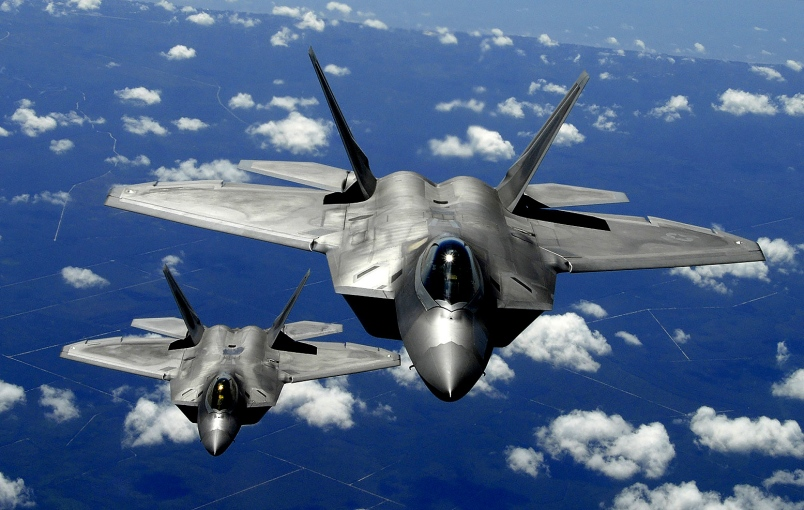
\includegraphics[height=.8\textheight]{raptor.jpeg}
     \caption{Lockheed F-22 Raptor}
\end{center}
\end{frame}



\begin{frame}\frametitle{Pourquoi????}


  \begin{figure}
\centering
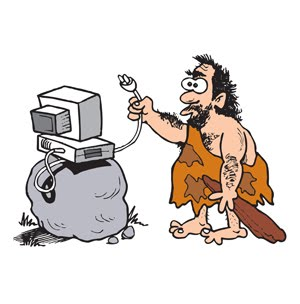
\includegraphics{caveman.jpg}
\caption{La France et l'enseignement de l'informatique}
\end{figure}
  
\end{frame}




\section{Organisation de l'année: que va-t-on étudier ?}

\begin{frame}
\protect\hypertarget{organisation-de-lannuxe9e-que-va-t-on-uxe9tudier}{}

Multiples facettes, multiples intervenants. Au programme sept thèmes qui
seront évoqués dans différents contextes tout au long de l'année:

\begin{itemize}
\tightlist
\item
  Internet
\item
  Web
\item
  Structuration des données
\item
  Réseaux sociaux
\item
  Cartes
\item
  Photos
\item
  Objets connectés
\end{itemize}

\end{frame}


\end{document}

%%% Local Variables:
%%% mode: latex
%%% TeX-master: t
%%% End:
